\section{Methoden}
	
	Dieser Abschnitt beschäftigt sich mit dem Aufbau der beiden Schaltkreise, sowie auch den Unsicherheiten welche bei diesem Versuch auftreten.
	
	\subsection{Aufbau}
		
		
		\subsubsection{Serienresonanzkreis}
			
			\begin{figure}[ht]
				\centering
				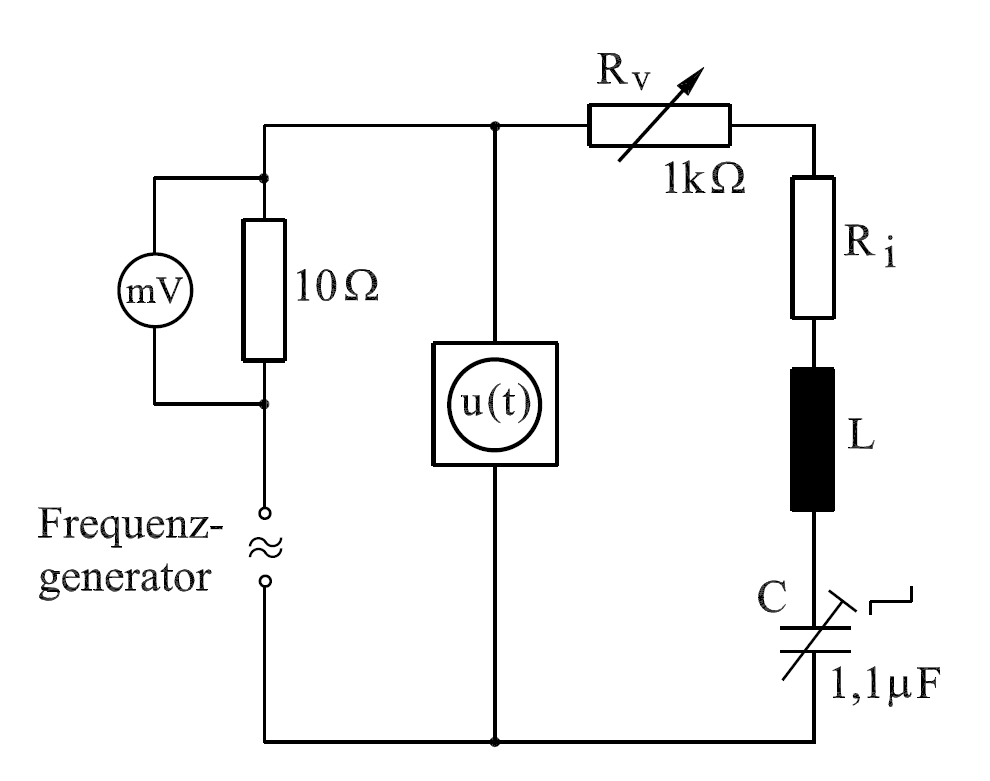
\includegraphics[width=0.9\textwidth]{auswertung/Serienresonanz.PNG}
				\caption{Schaltskizze für den Aufbau des in Serie geschalteten Schwingkreises.}
				\label{fig:SerienResonanzSkizze}	
			\end{figure}
			
			Für den Serienresonanzkreis wird der in Abb. \ref{fig:SerienResonanzSkizze} dargestellte Aufbau verwendet.
			Zu erkennen sind ein Frequenzgenerator, ein \SI{10}{\ohm} Widerstand, an dem ein Multimeter zur Messung der Spannung anliegt, ein Oszilloskop u$(t)$, welches parallel zu der Reihenschaltung von Kondensator $C$, Spule $L$ mit Innenwiderstand $R_\text{i}$ und einem bis zu \SI{1}{\kilo\ohm} regulierbaren Widerstand $R_\text{v}$.
			Der Frequenzgenerator dient als Wechselstromquelle, welcher auf eine feste Frequenz und Spannung eingestellt werden soll.
			 
			%TODO	?

		\subsubsection{Parallelresonanzkreis}
			
			\begin{figure}[ht]
				\centering
				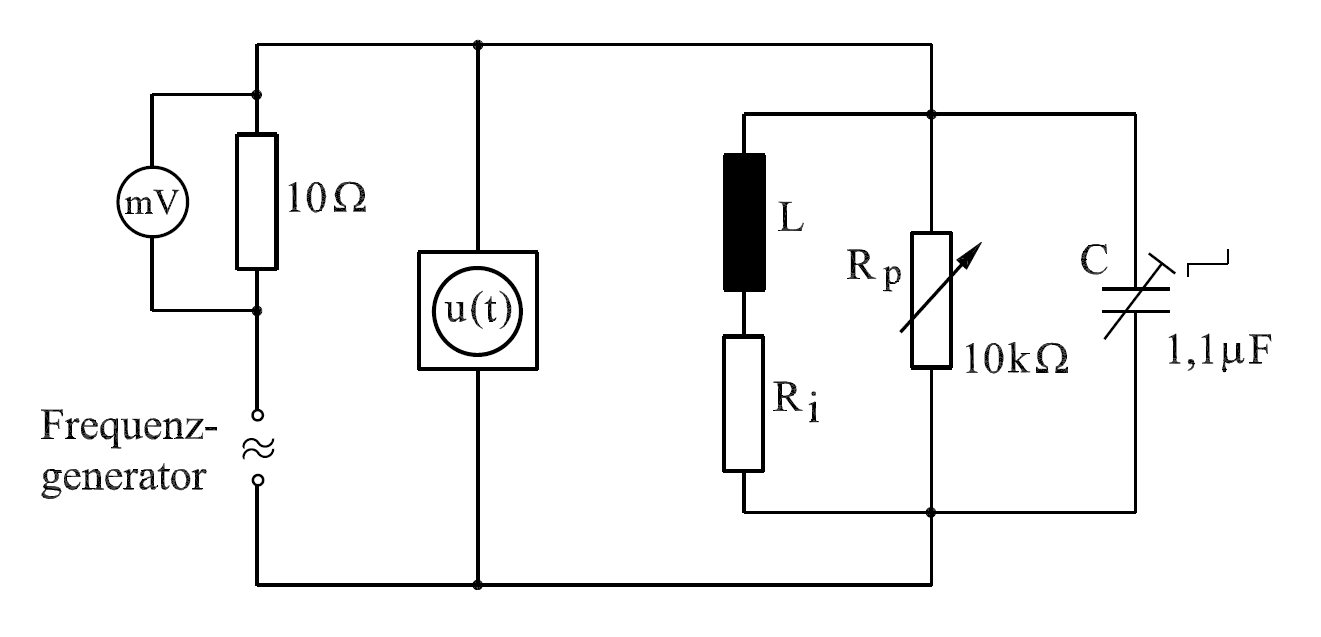
\includegraphics[width=0.9\textwidth]{auswertung/Parallelresonanz.PNG}
				\caption{Schaltskizze für den Aufbau des in Serie geschalteten Schwingkreises.}
				\label{fig:ParallelResonanzSkizze}	
			\end{figure}
			
			Der in Abb. \ref{fig:ParallelResonanzSkizze} dargestellte Schaltkreis für den Parallelresonanzkreis unterscheidet sich von dem Serienschaltkreis lediglich um die Parallelschaltung von Spule $L$ mit Innenwiderstand $R_\text{i}$, Kondensator $C$ und einem bis zu \SI{10}{\kilo\ohm} regulierbaren Widerstand $R_\text{p}$. 
			Dieser Block ist wie auch zuvor parallel zu dem Oszilloskop geschaltet.
			Hier wird die selbe Frequenz, wie auch für den Serienresonanzkreis verwendet, jedoch eine höhere Spannung.
			%TODO

	\subsection{Unsicherheiten} 

		Die bei diesem Versuch auftretenden Unsicherheiten setzen sich aus der Unsicherheit für den Kondensator $U_\text{c}$, für die digitale Anzeige des Multimeters $U_\text{digital}$, ... %TODO
		Die Berechnung der kombinierten Unsicherheiten erfolgt nach GUM und ist im Anhang aufgeführt.

\section{Durchführung und Datenanalyse}

	Zur Bestimmung der Resonanzkurve $I(f)$, wird die Stromstärke $I$ in den Schaltkreisen über die gemessenen Spannung und die vorliegenden Widerstände bzw. Impedanzen ermittelt.
	Dazu dienen folgende Formeln:
	
	%TODO
	
	Die verwendete Frequenz der Wechselstromquelle für beide Schwingkreise betrug \SI{1000}{\hertz}.
	Für die Eingangspannungen wurden für den Serienresonanzkreis \SI{2}{\volt} und \SI{5}{\volt} für den Parallelresonanzkreis verwendet.
	Es wurden für verschiedene Widerstände $R_\text{v}$ (Serie, mit \SI{0}{\ohm}, \SI{200}{\ohm} und \SI{500}{\ohm}) und $R_\text{p}$ (parallel, mit $\infty$\si{\ohm} \SI{2}{\kilo\ohm} und \SI{10}{\kilo\ohm}) Messungen in Abhängigkeit der Kapazität des Kondensators $C$ durchgeführt.
\section{Diskussion}

	%TODO



